
%Preamble
\documentclass[twoside]{article}
\usepackage{mdframed}
\usepackage[hmarginratio=1:1,top=32mm,columnsep=20pt]{geometry} % Document margins
\usepackage{multicol} % Used for the two-column layout of the document
\usepackage[hang, small,labelfont=bf,up,textfont=it,up]{caption} % Custom captions under/above floats in tables or figures
\usepackage{booktabs} % Horizontal rules in tables
\usepackage{colortbl}
\usepackage{float} % Required for tables and figures in the multi-column environment - they need to be placed in specific locations with the [H] (e.g. \begin{table}[H])
\usepackage{hyperref} % For hyperlinks in the PDF
\usepackage[final]{pdfpages}
\usepackage{amsmath,amsthm,amssymb}
\usepackage{lettrine} % The lettrine is the first enlarged letter at the beginning of the text
\usepackage{paralist} % Used for the compactitem environment which makes bullet points with less space between them
\usepackage{tikz}
\usepackage{esint}
\usepackage{centernot}
\usepackage{afterpage}
\usepackage{lmodern}
\usetikzlibrary{3d}
\usetikzlibrary{patterns,calc,hobby}
\usetikzlibrary{decorations.pathreplacing}
\tikzset{
	partial ellipse/.style args={#1:#2:#3}{
		insert path={+ (#1:#3) arc (#1:#2:#3)}
	}
}
%\usepackage{xcolor}
\usepackage{geometry}
\usepackage{graphicx}
\usepackage{fancyhdr} % Headers and footers
\pagestyle{fancy} % All pages have headers and footers
\fancyhead{} % Blank out the default header
\fancyfoot{} % Blank out the default footer
\fancyhead[C]{Jimmy Yue $\bullet$ Visual Analytics $\bullet$ Jimmy Yue} % Custom header text
\fancyfoot[RO,LE]{\thepage} % Custom footer text

\usepackage{xcolor}
\newmdenv[skipabove=7pt,
rightline=false,
leftline=true,
topline=false,
bottomline=false,
skipbelow=5pt,
linecolor=black,
innerleftmargin=5pt,
innerrightmargin=5pt,
innertopmargin=5pt,
leftmargin=0cm,
rightmargin=0cm,
linewidth=4pt,
innerbottommargin=5pt]{cBox}

\theoremstyle{definition}
\newtheorem*{solutionT}{Solution}

\newenvironment{solution}{\begin{cBox}\begin{solutionT}}{\hfill{\scriptsize\ensuremath{\square}}\end{solutionT}\end{cBox}}

%%%%%%%%%%%%%%%%%%%%%%%%%%%%%%%%%%%%%%%%%%%%%%%%%%%%%%%%%%%%%%%%%%%%%%%%%%%%%%%%%%%%%%%%%%%%
\newcommand{\vect}[1]{\vec{\pmb{#1}}}
\newcommand{\uvect}[1]{\hat{\mathbf{#1}}}
\newcommand{\leviciv}{\epsilon_{ijk}}

\newmdenv[skipabove=7pt,
rightline=false,
leftline=true,
topline=false,
bottomline=false,
skipbelow=5pt,
linecolor=black,
innerleftmargin=5pt,
innerrightmargin=5pt,
innertopmargin=5pt,
leftmargin=0cm,
rightmargin=0cm,
linewidth=4pt,
innerbottommargin=7,
backgroundcolor=light-gray]{dBox}



\theoremstyle{definition}
\newtheorem*{proof1}{Definition}

\newenvironment{ddef}{\begin{dBox}\begin{proof1}}{\hfill{\scriptsize}\end{proof1}\end{dBox}}
\newcommand{\pdif}[2]{\frac{\partial#1}{\partial#2}}
\definecolor{light-gray}{gray}{0.85}
%----------------------------------------------------------------------------------------
%-	TITLE SECTION
%----------------------------------------------------------------------------------------

\title{\vspace{-15mm}\fontsize{24pt}{10pt}\selectfont\textbf{Assignment 1}} % Article title

\author{
\large
\textsc{Jimmy Tsz Ming Yue}\thanks{440159151}\\[2mm] % Your name
\normalsize University of Sydney \\ % Your institution
\normalsize \href{mailto:jyue6728@uni.sydney.edu.au}{jyue6728@uni.sydney.edu.au} % Your email address
\vspace{-5mm}
}
\date{}

%----------------------------------------------------------------------------------------
\newlength{\classpageheight} \setlength{\classpageheight}{\pdfpageheight}
\newlength{\classpagewidth} \setlength{\classpagewidth}{\pdfpagewidth}

\begin{document}

\maketitle % Insert title

\thispagestyle{fancy} % All pages have headers and footers
\hrule \smallskip

\noindent Semester 2 \quad Visual Analytics\hspace{9.5cm} 2018

\hrule

\vspace{1cm}
{\large\textbf{Assignment/Project Coversheet - Individual Assessment}}\\
\\
\textbf{Unit of Study}: COMP5048 Visual Analytics\\
\\
\textbf{Assignment Name}: Assignment 1 - Graph Drawing\\
\\
{\large\textbf{DECLARATION}}\\
I declare that I have read and understood the University of Sydney Academic Dishonesty
and Plagiarism in Coursework Policy, and except where specifically acknowledged, the
work contained in this assignment/project is my own work, and has not been copied from
other sources or been previously submitted for award or assessment.
I understand that failure to comply with the the Academic Dishonesty and Plagiarism in
Coursework Policy, can lead to severe penalties as outlined under Chapter 8 of the
University of Sydney By-Law 1999 (as amended). These penalties may be imposed in
cases where any significant portion of my submitted work has been copied without proper
acknowledgement from other sources, including published works, the internet, existing
programs, the work of other students, or work previously submitted for other awards or
assessments.
I realise that I may be asked to identify those portions of the work contributed by me and
required to demonstrate my knowledge of the relevant material by answering oral
questions or by undertaking supplementary work, either written or in the laboratory, in
order to arrive at the final assessment mark.\\
\\
\textbf{Student ID}: 440159151\\
\\
\textbf{Student Name}: Jimmy Tsz Ming Yue\\
\\
\textbf{Signed}:
\begin{figure}[h]
	\includegraphics[scale=0.15]{signature.png}
\end{figure}
\\ 
\textbf{Date}: 11/09/201

\newpage
\includepdf{w2.pdf}
\newpage
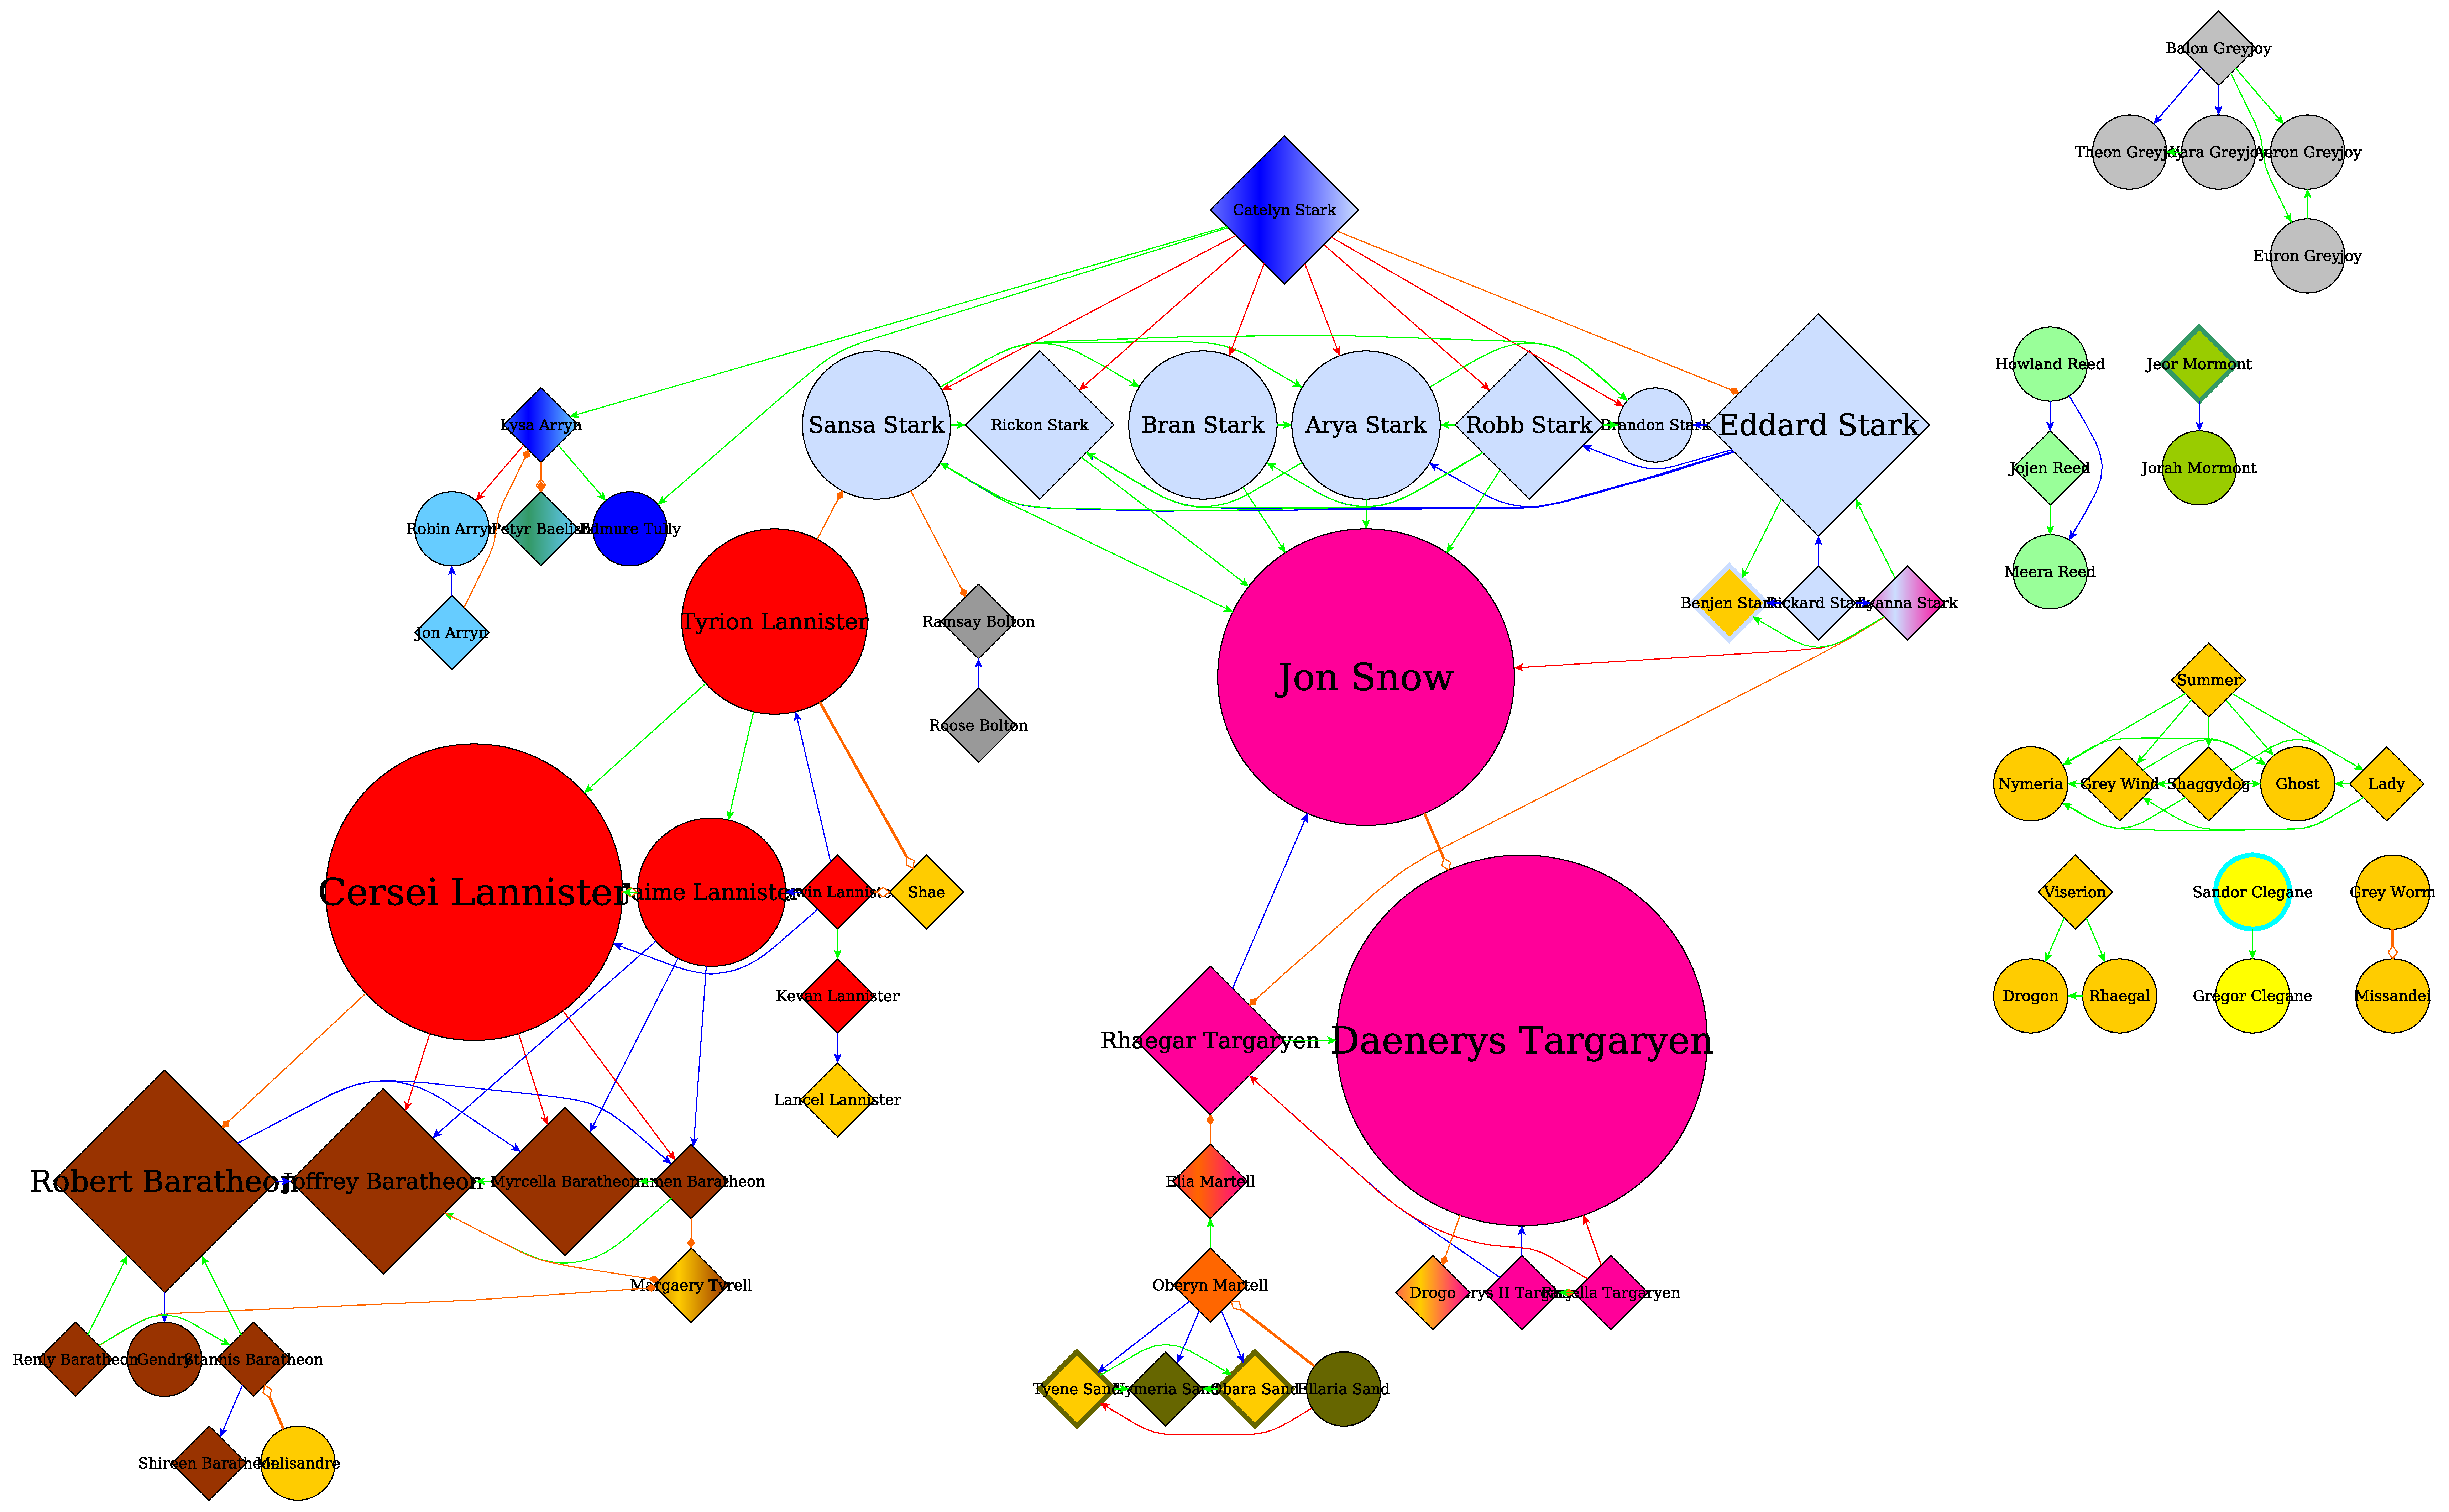
\includepdf{ohana.pdf}
\newpage
\includepdf{alle.pdf}
\section{Game of Thrones Visualisation}
\subsection{Main Visualisation}
\subsubsection{Legend}
\begin{enumerate}
	\item Node Shape representing Character Status
		\begin{enumerate}
			\item Diamond: Dead
			\item Circle: Alive
		\end{enumerate}
	\item Node Fill Colour representing House by Birth, with mixed colours representing marriage to that house.
		\begin{table}[h!]
			\centering
			\caption{House Colour Legend}
				\begin{tabular}{ll}
				House       & Fill Colour              \\  \hline
			Baelish     & \cellcolor[HTML]{339966} \\
		Arryn       & \cellcolor[HTML]{66CCFF} \\
	Baratheon   & \cellcolor[HTML]{993300} \\
Bolton      & \cellcolor[HTML]{999999} \\
Clegane     & \cellcolor[HTML]{FFFF00} \\
Dayne       & \cellcolor[HTML]{CC99FF} \\
Dondarrion  & \cellcolor[HTML]{993366} \\
Frey        & \cellcolor[HTML]{3366FF} \\
Greyjoy     & \cellcolor[HTML]{C0C0C0} \\
Lannister   & \cellcolor[HTML]{FF0000} \\
Martell     & \cellcolor[HTML]{FF6600} \\
Mormont     & \cellcolor[HTML]{99CC00} \\
Payne       & \cellcolor[HTML]{FFFF99} \\
Reed        & \cellcolor[HTML]{99FF99} \\
Stark       & \cellcolor[HTML]{CCDEFF} \\
Targaryen   & \cellcolor[HTML]{FF0099} \\
Tarth       & \cellcolor[HTML]{33CCCC} \\
Thorne      & \cellcolor[HTML]{FFCC99} \\
Tully       & \cellcolor[HTML]{0000FF} \\
Sand Snakes & \cellcolor[HTML]{666600}
\end{tabular}
\end{table}
\item Node Border colours to represent groups:
	% Please add the following required packages to your document preamble:
	% \usepackage[table,xcdraw]{xcolor}
	% If you use beamer only pass ``xcolor=table'' option, i.e. \documentclass[xcolor=table]{beamer}
	\begin{table}[h!]
		\centering
		\caption{Groups Legend}
			\begin{tabular}{ll}
			Group                       & Border Colour            \\ \hline
		Brotherhood Without Banners & \cellcolor[HTML]{00FFFF} \\
	Free Folk                   & \cellcolor[HTML]{FF3300} \\
House Stark                 & \cellcolor[HTML]{CCDEFF} \\
Night's Watch               & \cellcolor[HTML]{339966} \\
Sand Snakes                 & \cellcolor[HTML]{666600}
\end{tabular}
\end{table}


	\item Edge colours, line type and arrow type  to represent relationship types:
		\begin{table}[h!]
			\centering
			\caption{Edge Legend}
			\begin{tabular}{llll}
			Relationship & Edge Colour              & Edge Type & Arrow Type        \\ \hline
		Sibling      & \cellcolor[HTML]{00FF00} & thin      & normal arrow      \\
	Father       & \cellcolor[HTML]{0000FF} & thin      & normal arrow      \\
Mother       & \cellcolor[HTML]{FF0000} & thin      & normal arrow      \\
Lover        & \cellcolor[HTML]{FF6600} & thin      & unfilled diamond  \\
Spouse       & \cellcolor[HTML]{FF6600} & thin      & filled diamond    \\
Allegiance   & \cellcolor[HTML]{000000} & thick     & unfilled triangle \\
Killed       & \cellcolor[HTML]{000000} & dashed    & normal arrow     
\end{tabular}
\end{table}
\end{enumerate}
\subsubsection{Preparation}
Visualisation was created using yed, for which the provided graphml was imported. It is noted that editing of the source was done via vim to ensure correct importation of edges via addition of 
\begin{verbatim}
for = ``edges''
\end{verbatim}
in the relation and type sections of the provided graph information. As the visualisation at the current moment is poor, different layouts were tried (organic, hierachy etc) for which a radial setting with wide node dispersal was observed to be the best fit. This is due to the clarity in node positioning with minimial edge crossings whilst preserving this node clarity. Then the status of the characters (either dead or alive) were differentiated through selecting nodes possessin these qualities, and assigning a node shape for clarity (diamond = dead), (circle = alive). Then using the yed property mapper, all the above line, colour assignments were done. Then reflecting the amount of directed incoming edges on nodes, the nodes were resized to show weights.

\subsubsection{Strengths and Weakness}
There are some key strengths in the above visualisation, with the relationships between each individual explicitly showna and the node placements highlighting key members (Danerys, Jon Snow). Despite this the visualisation possess multiple edge crossings which is not desired. This was attempted to be mitigated through different edge colourings between differing relationship types, however it should still be considered. To make these clearer the subgraphs shown above (page 3 and 4) show clearly the familial and love ties and the allegiance as an attempt to further elucidate these relationships
\subsection{Familial and Love Ties}
\subsubsection{Legend} 
Same as Main visualization
\subsubsection{Preparation}
Using the yed object selection tool, and searching up erroneous relation types such as; allegiance and killed we can generate the familial and love ties between characters. A directed tree highlighted this relationships very clearly. 
\subsubsection{Strengths and Weaknesses}
\begin{enumerate}
	\item Very Clear familial and love ties shown
	\item excluded some characters who did not possess these ties, and did not show allegiances
	\item Generated Four Seperate Trees
\end{enumerate}
\subsection{Allegiance}
\subsubsection{Legend}
Same as Main
\subsubsection{Preparation}
Using the object selection tool off the main graph and searching up erroneous relation typs such as father mother sibling killed spouse lover, a visualization of the flow of allegiance can be generated. 
\subsubsection{Strengths and Weaknesses}
\begin{enumerate}
	\item Very Clear allgegiances shown
	\item excluded some characters who did not have allegiances 
	\item missing familial data 
	\item Generated many small trees 
\end{enumerate}
\newpage
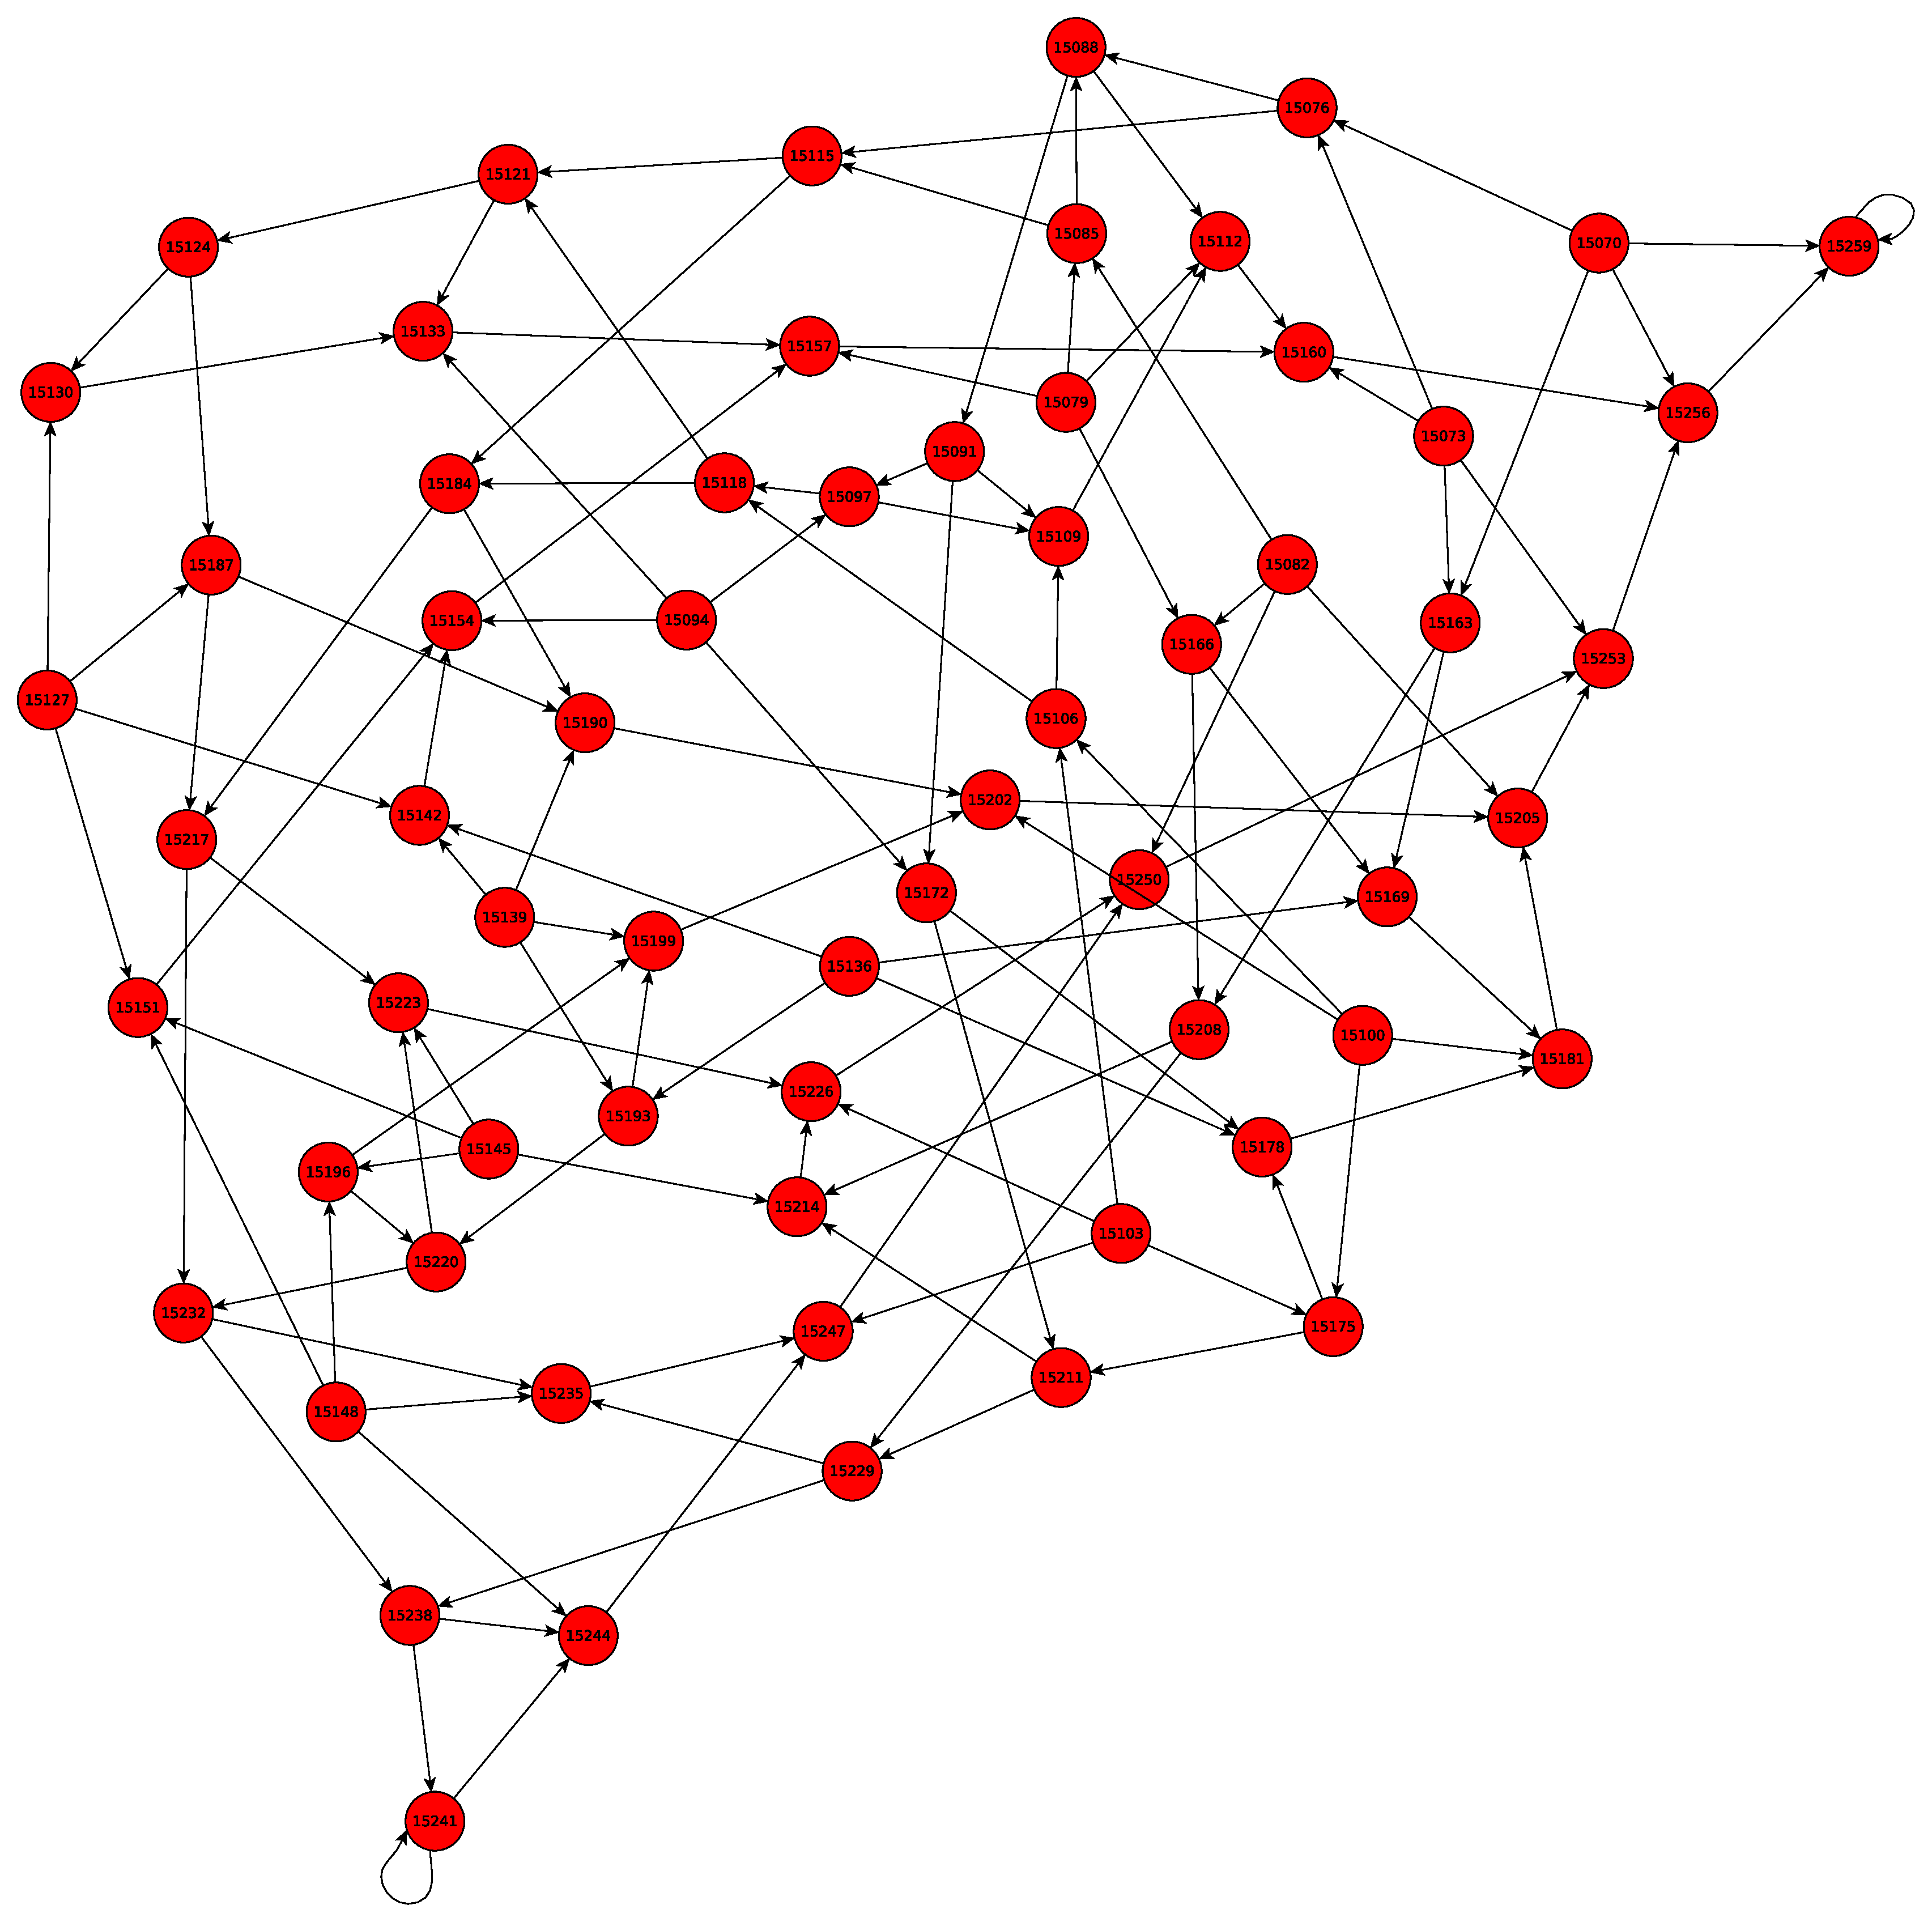
\includepdf{gd99b.pdf}
\newpage
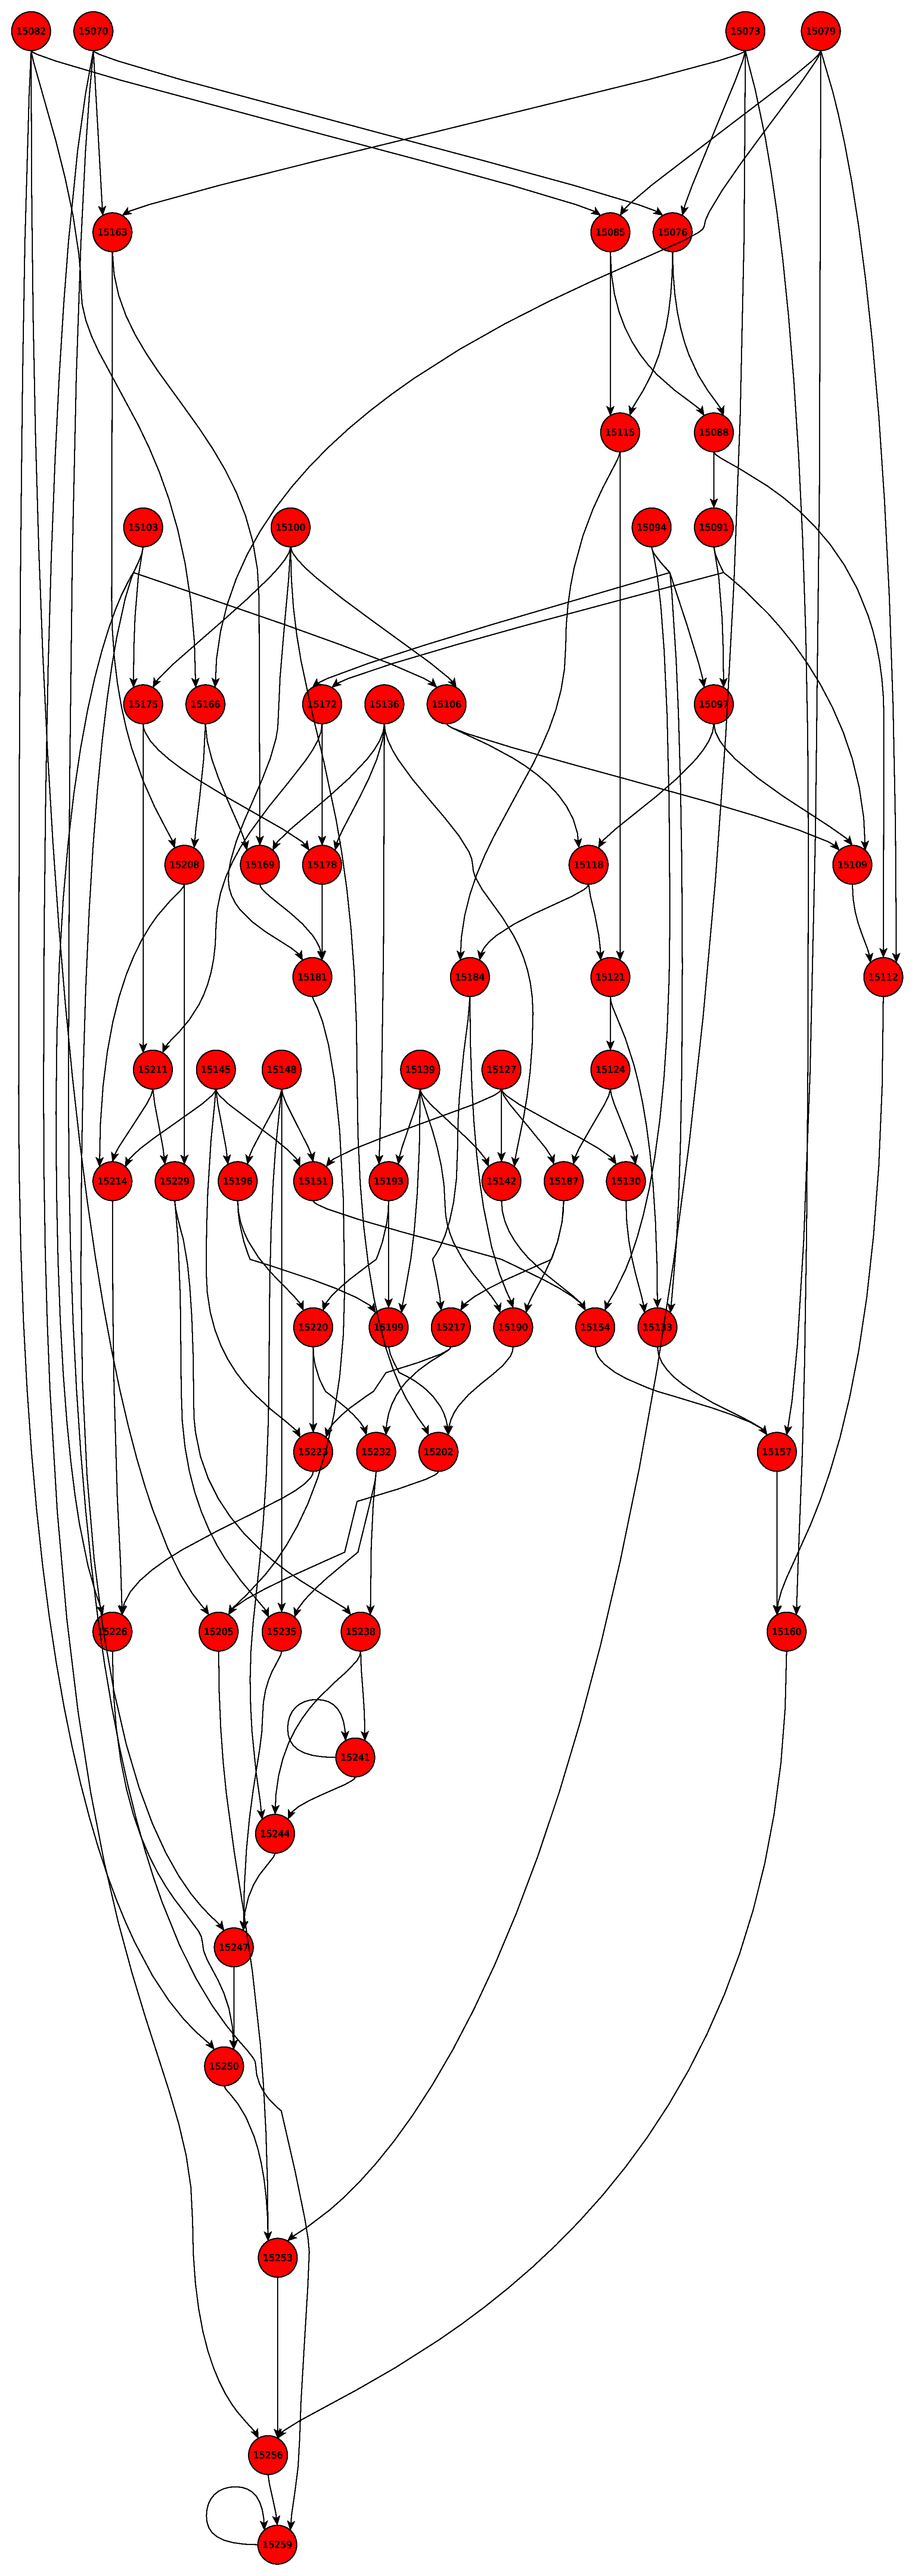
\includepdf{gd99b2.pdf}
\newpage
\section{Graph Drawing Contest 1999 B Visualisation}
\subsection{Organic Layou}
\subsubsection{Preparation}
The graph was constructed using yed. Multiple layouts were attempted in the beginning of the processas the importation yielded a very cluttered very messy layout comprised of multiple edge crossings.  After multiple trial and error patterns, an organic layout was selected. This was not particularly good as the spacing of the nodes were very poor and multiple edge crossing were evident. Furthermore there was no clear indication of two nodes with a self directed edge. After some parameter adjustments such as enabling the options of avoiding edge node overlap and compactness arguments under an aspect ratio restriction, the above visualization was produced after node enlargement and coloring  which clearly highlights the nodes with self directed edges 15259 and 15241.

\subsubsection{Strengths and Weaknessess}
\begin{enumerate}
	\item Very Clear edges and layout with compact drawin
	\item Could possibly generate a more regularized graph shape with lesser edge crossings (which seemed impossible with yed) 
	\item  Does not show a clear network flow and has upward pointing arrows with no layering
\end{enumerate}

\subsection{Hierachical Directed Graph}
\subsubsection{Preparation}
We provide an alternative visulaisation as according to the parameters in the lecture slides. This was done via hiearchical layout generation with specificed layering. 
\subsubsection{Strengths and Weaknessess}
\begin{enumerate}
	\item Directed Graph format as in the lectures with downwards pointing arrows and clear layering shown 
	\item Confusing non-compact layout with multiple crossings that are suboptimal
\end{enumerate}
\end{document}
